%%%%%%%%%%%%%%%%%%%%%%%%%%%%%%%%%%%%%%%%%%%%%%%%%%%%%%%%%%%%%%%%%%%%%%%%%
%Objetivo: Realizar uma pesquisa com profissionais envolvidos em manutenção de
%		   software a fim de verificar a situação atual das funcionalidades
%		   oferecias pelas FGRM.
%Autor: Vagner Clementino<vagnercs@dcc.ufmg.br> e
%		Rodolfo Resende<rodolfo@dcc.ufmg.br>
%Data Criação: sex fev  3 19:57:56 BRST 2017
%Data Modificação: sex fev  3 19:58:14 BRST 2017
%Data Revisão: sex fev  3 19:58:24 BRST 2017
%%%%%%%%%%%%%%%%%%%%%%%%%%%%%%%%%%%%%%%%%%%%%%%%%%%%%%%%%%%%%%%%%%%%%%%%%%
\chapter{Pesquisa com Profissionais: Conhecendo e Melhorando as Funcionalidades
das FGRM's}
\label{ch:pesquisa-profissionais}

\section{Introdução}
\label{sec:pesquisa-profissionais-intro}

Uma pesquisa baseada em questionários, conhecido na literatura como
\textit{Survey}, é uma abordagem de coleta e análise de dados na qual os
participantes respondem a perguntas ou declarações que foram desenvolvidas
antecipadamente~\cite{kasunic2005designing}. Este tipo de pesquisa se divide em
duas grandes principais: questionários auto-administrados e
entrevistas~\cite{kasunic2005designing}. O primeiro tipo é aquele que  a maioria
das pessoas pensa quando falamos em  ``pesquisa de opinião'', no qual geralmente
recebemos por meio de correio eletrônico ou estão disponíveis através de páginas
da Internet. As entrevistas apresentam as mesmas características dos
questionários auto-administrados, sendo que a principal diferença consiste na
profundidade que as perguntas são apresentadas aos participantes.  Neste estudo
utilizamos um questionário auto-administrado como instrumento de coleta dos
dados.

Em uma pesquisa baseada em questionário, quando conduzida adequadamente, permite
que os pesquisadores generalizem as crenças e opiniões de uma população mediante
os dados coletados de um subconjunto do público-alvo (amostra). No trabalho
conduzido por Kasunic~\cite{kasunic2005designing} são apresentadas um conjunto
de etapas a serem seguidas no processo de condução deste tipo de trabalho
acadêmico:

\begin{enumerate}
\item{Identificar os objetivos da pesquisa}
\item{Identificar e caracterizar o público-alvo}
\item{Elaborar o plano de amostragem}
\item{Elaborar e escrever um questionário}
\item{Aplicar questionário de teste ou piloto}
\item{Distribuir o questionário}
\item{Analisar os resultados e escrever o relatório}
\end{enumerate}

Em uma série de artigos~\cite{pfleeger2001principles,pfleeger2002principles},
Kitchenham e Pfleeger discutem os princípios da pesquisa com questionário no
âmbito da Engenharia de Software (ES). O foco daquele estudo esteve
principalmente nas etapas 3, 4, 6 e 7 do estudo feito por
Kasunic~\cite{kasunic2005designing}. Os autores apresentam conceitos básicos de
estatística para discutir algumas questões relativas à população e amostra.
Nestes mesmos estudos os autores investigaram o desenho de quatro levantamentos
na área de ES e concluem que em apenas um deles foi composto por uma amostra
significativa da população. Ao final eles salientam a necessidade que este tipo
de estudo científico utilize uma metodologia concisa de modo a reduzir qualquer
viés no tocante à amostra utilizada.

Com o objetivo de coletar os aspectos mais importantes das funcionalidades
oferecidas pelas Ferramentas de Gerenciamento de Requisições de Mudança (FGRM),
do ponto de vista dos profissionais ligados à manutenção de software, foi
realizada um levantamento com profissionais (survey). O planejamento e o desenho
da pesquisa seguiu as diretrizes propostas nos trabalhos de
Wohlin~\cite{wohlin2012experimentation} e Kasunic~\cite{kasunic2005designing}.
Em especial, no tocante a definição da população e da amostra de interesse
utilizamos o arcabouço (framework) proposto por De Mello e
outros~\cite{de2015investigating, de2014towards}.

A população da pesquisa é a comunidade envolvida com o processo de manutenção de
software e que faça uso de FGRM's. Neste sentido, utilizamos  como amostra os
profissionais que estão envolvidos no projeto de código aberto
Python\footnote{\url{http://bugs.python.org/}}. Por outro lado, visando alcançar
os profissionais que trabalham em empresas privadas, utilizamos profissionais
que fazem parte da rede social de desenvolvedores Stack
Overflow\footnote{\url{http://stackoverflow.com}}. Neste caso estamos
interessados no usuários da rede que tenham participado de discussões na rede de
assuntos relacionados à manutenção de software. A pesquisa foi replicada em uma
empresa pública de software do qual o autor possui vínculo.  Maiores detalhes
sobre o processo de escolha das amostras serão discutidos posteriormente.

A importância deste tipo de trabalho está na possibilidade de avaliar se as
pesquisas relativas a evolução das funcionalidades das FGRM's estão em
consonância com as necessidades dos profissionais envolvidos em manutenção de
software, reduzindo, desta forma, a distância entre o estado da arte e o estado
da prática.

\section{Objetivo da Pesquisa com Profissionais}
\label{sec:objetivo_da_pesquisa_com_profissionais}

Em linhas gerais, o objetivo desta etapa do estudo é analisar, através da
percepção e opinião dos profissionais envolvidos em manutenção de software, a
situação das funcionalidades atualmente oferecidas pelas FGRM's, bem como
a adotação das metodologias propostos pelos agilistas no processo de manutenção
de software.

Para uma melhor apresentar a finalidade desta parte da dissertação estruturamos
o objetivo conforme propõe a metodologia GQM (Goal, Question e
Metric)\cite{gqm}, \textit{o propósito deste estudo avaliar as funcionalidades
	oferecidas pelas FGRM's e as melhorias propostas nas literatura para este
	tipo de ferramenta, do ponto de vista dos profissionais envolvidos em
	manutenção de software no contexto de projetos de software de código aberto
	e uma empresas publicas e privadas de informática.}

Com intuito de atingir os objetivos propostos fora definidas as seguintes
questões de pesquisa:

\begin{description}
	\item[Questão 01] Qual a opinião dos profissionais envolvidos em Manutenção
		de Software com relação as funcionalidades oferecidas atualmente pelas
		FGRM\@?
	\item[Questão 02] Na visão dos profissionais envolvidos em Manutenção de
		Software quais das extensões propostas na literatura teriam maior
		relevância em suas atividades atuais?
	\item[Questão 03] Como as práticas propostas pelos agilistas estão sendo
	utilizadas especialmente no processo de manutenção de software?
	\item[Questão 04] Como as FGRM's podem ajudar aos times devotados à manutenção
	de software na prática adotada pelos agilistas?
\end{description}

As questões de pesquisas foram respondidas mediante a realização de uma pesquisa
baseada em questionário (survey). O desenho da pesquisa é detalhada na próxima
seção onde discutimos a estrutura do questionário bem como a amostra a população
que foi utilizada.

\section{Desenho e Metodologia da Pesquisa com Profissionais}
\label{sec:desenho_da_pesquisa_com_profissionais}

\subsection{Conceitos Básicos}

Estudos primários em Engenharia de Software (SE), como os levantamentos
(surveys), são muitas vezes conduzidos em amostras estabelecidas por
conveniência~\cite{sjoberg2005survey, dybaa2006systematic}. Vale ressaltar que
neste tipo de abordagem são necessários esforços consideráveis, contudo, a
generalização dos resultados é limitada, mesmo quando as características de
outros estudos são claramente descrito e repetidos~\cite{de2015investigating}.
Em resumo, o fato do pesquisador utilizar uma metodologia já consagrada para
realização de pesquisas com questionários é importante que se priorize a escolha
da população de interesse e de suas respectivas amostras.

Um desafio no estabelecimento de amostras representativas nos levantamentos com
questionários em Engenharia de Software inclui a identificação de fontes
relevantes e disponíveis a partir das quais podem ser estabelecidas estruturas
de amostragem~\cite{de2014towards}. Neste contexto, uma alternativa aos
pesquisadores é a utilização de fontes alternativas tipicamente disponíveis na
Internet para aumentar o tamanho da amostra, como as redes
sociais~\cite{de2013would}. Uma outra fonte de dados que pode aumentar a
significância das amostras são os projetos de código aberto e os seus diversos
artefatos disponíveis na rede.

Esta Pesquisa com Profissionais (survey) consistiu de um estudo exploratório sem
uma hipótese prévia a ser avaliada. Conforme discutido anteriormente, a
população de interesse desta pesquisa é composta por profissionais envolvidos em
desenvolvimento e manutenção de software. Para sistematizar o processo de
escolha da amostragem utilizamos o arcabouço (framework) conceitual proposto por
de Mello e outros~\cite{de2014towards} que está representado na
Figura~\ref{fig:framework-amostragem}. O modelo proposto inclui além dos
conceitos estatísticos tradicionalmente utilizados em pesquisas por questionário
, tais como público-alvo, população, amostragem e unidade de
observação~\cite{thompson2012sampling}, introduz um conjunto de novos conceitos
que visam apoiar o processo de escolha da amostragem em questionários,
especialmente em ES\@. Os conceitos que os autores propuserem incluem:
\textit{Fonte de Amostragem, Unidade de Pesquisa, Plano de Pesquisa e Estratégia
	de Amostragem}.

\begin{figure}[htpb]
	\centering
	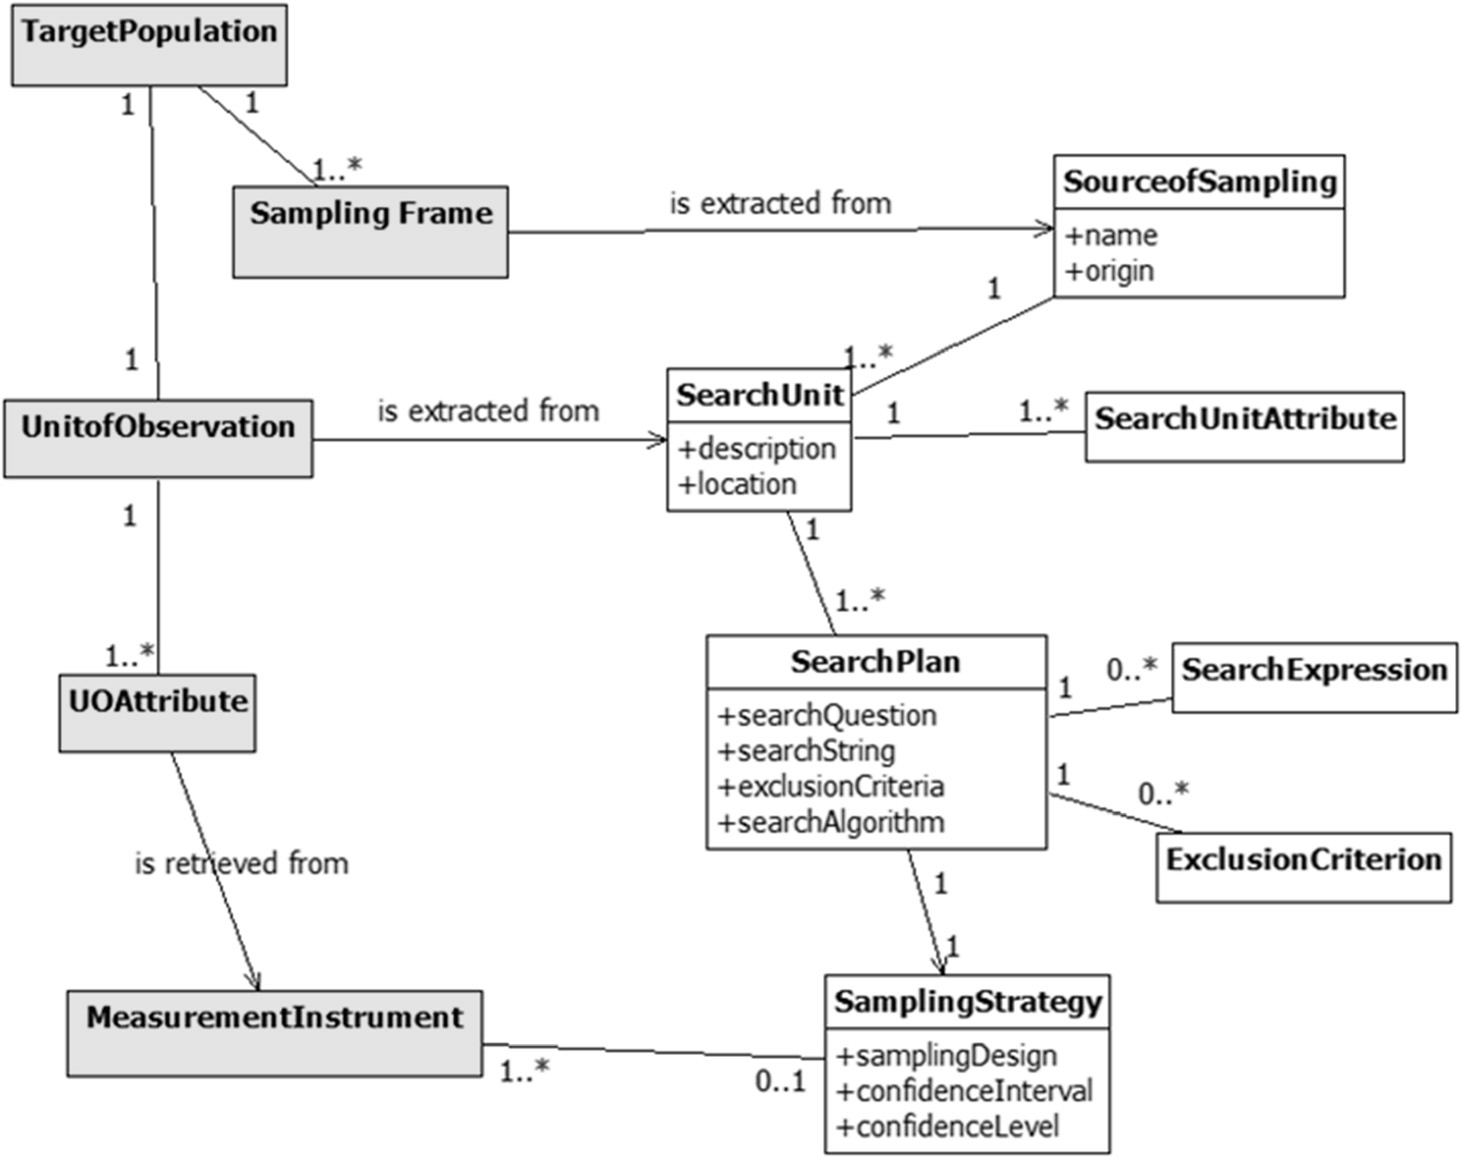
\includegraphics[width=0.8\linewidth]{./chapter-pesquisa-com-profissionais/img/framework-amostragem.png}
	\caption{Os conceitos que compõem o Arcabouço Conceitual proposto por de
		Mello. Extraído de~\cite{de2015investigating}}
\label{fig:framework-amostragem}
\end{figure}

Uma \textit{Unidade de Observação} é a entidade que é estudada em determinado
experimento~\cite{wohlin2012experimentation}. Uma Unidade pode ser produtos,
processos, recursos, modelos, métricas, teorias ou pessoas. Uma \textit{Unidade
	de Pesquisa} caracteriza como uma ou mais \textit{Unidade de Observação}
podem ser recuperadas de uma \textit{Fonte de Amostragem} específica. O
\textit{Plano de Pesquisa} descreve como \textit{Unidades de Pesquisa} serão
sistematicamente recuperadas de uma Fonte de Amostragem e avaliadas para compor
a amostragem da pesquisa. Finalmente, a Estratégia de Amostragem descreve as
etapas que devem ser seguidas para definição da amostragem e recrutamento de
indivíduos que participarão do estudo.

Uma \textit{Fonte de Amostragem} consiste de um banco de dados, que não
necessariamente é automatizado, em que um subconjunto válido do público-alvo
pode ser sistematicamente recuperado, além de permitir a extração aleatória de
amostra da população de interesse. Sendo assim, os autores~\cite{de2014towards}
afirmam que no caso de determinada Fonte de Amostragem ser considerada válida
para um contexto de pesquisa específico, pode-se concluir que as amostras podem
ser extraídas desta fonte a fim de serem utilizados no mesmo contexto de
pesquisa. Para ser considerada válida, uma Fonte de Amostragem deve satisfazer,
pelo menos, os seguintes Requisitos Essenciais (Essential Requirements\@-\@ ER):

\begin{description}
	\item[ER1] Uma Fonte de Amostragem não deve representar intencionalmente um
		subconjunto segregado do público-alvo, ou seja, dado um público-alvo
		\textit{``X''}, não seria adequado pesquisar por unidades na Fonte
		intencionalmente desenhada para compor um subconjunto específico de
		\textit{``X''}.
	\item[ER2] Uma Fonte de Amostragem não deve apresentar qualquer viés em
		incluir na sua base de dados determinados subconjuntos do público-alvo.
		Critérios desiguais para inclusão de Unidades de Pesquisa significam
		oportunidades desiguais para oportunidades de amostragem.
	\item[ER3] Todas as Unidades de Pesquisa das amostras e suas Unidades de
		Observação devem identificados por de forma única.
	\item[ER4] Todas as amostragem de determinada Unidade de Pesquisa devem ser
		acessíveis. Se houver unidades de pesquisa ocultas, não é possível
		contextualizar a população.
\end{description}

O estudo realizado por de Mello~\cite{de2014towards} cita outros requisitos que
são definidos como desejáveis que estão relacionados com amostragem, clareza e
integridade da amostra. 

\subsection{Metodologia}
\label{subsec:pesq_metodologias}
No caso desta pesquisa, o público-alvo é composto por profissionais devotados em
desenvolvimento e manutenção de software. O perfil do participante da população
de interesse é bastante geral, uma vez que um conjunto de características e
práticas deste tipo de profissional é bastante diversa e pode depender de
questões como processo de software utilizado, linguagem de programação
utilizada, tipo de projeto no qual está envolvido, dentre outras. Assim, todos
os profissionais que trabalham em projetos de software, sejam estes projetos de
código aberto ou de empresas privadas, podem potencialmente contribuir com esta
investigação. É importante destacar que cabe ao Plano de Pesquisa avaliar quando
a relevância do participante utilizando, por exemplo, o nível de experiência do
respondente como critério de inclusão. As subseções a seguir descrevem a
estratégia de recrutamento projetada para a pesquisa com profissionais
realizada neste estudo.

\subsubsection{Fonte de Amostragem, Unidade de Pesquisa e População}
\label{subsubsec:fontes_amostragem}

Para a realização deste estudo foi estabelecida 02 diferentes Fontes de
Amostragem conforme exibido na Tabela~\ref{tab:fontes-amostragens}. Estas fontes
foram selecionadas de modo a incluir profissionais que estão se dedicam a
projetos de código aberto (Python) e aqueles que possivelmente façam parte de
empresas privadas de desenvolvimento e manutenção de software (Stack Overflow).
Para o primeiro grupo, escolhemos um projetos de código aberto que tivessem pelo
menos 5 anos de existência, possuem uma comunidade bem estabelecida e permitam
acesso aos dados históricos das Requisições de Mudanças (RM). Para alcançarmos
os profissionais que trabalham em empresas privadas de desenvolvimento de
software utilizamos uma rede social composto em sua maioria por desenvolvedores
(Stack Overflow). Este rede social foi  selecionada especialmente por conta de
sua cobertura, que conta com mais de 6 milhões de
usuários~\footnote{\url{http://stackexchange.com/sites}}.

\begin{table}[htb]
\centering
\resizebox{\textwidth}{!}{%
\begin{tabular}{|llc|}
\hline
\multicolumn{1}{|c}{\textbf{Fonte de Amostragem}} & \multicolumn{1}{c}{\textbf{URL}}                & \textbf{Membros} \\ \hline
Python                                            & https://bugs.python.org/                        & $\sim$19 K       \\
LinkedIn                                           & https://www.linkedin.com/                       & $\sim$347 M      \\
\end{tabular}%
}
\caption{Fontes de Amostragem utilizadas no estudo.}
\label{tb:fonte-de-amostragens}
\end{table}

No escopo deste estudo, para o projeto de código aberto utilizado, a lista de
Requisições de Mudanças serão a Unidade de Pesquisa a ser considerada. No caso
da rede social Stack Overflow foi considerada cada discussão proposta por um
usuário (thread) como a Unidade de Pesquisa. Em todas as Fontes de Amostragem
foram coletados os seguintes atributos: \textit{Nome do Participante, E-mail do
	Participante, Data de Interação e Tipo de Interação}. No caso do Stack
Overflow utilizamos um métrica adicional da própria rede social conhecida como
reputação~\footnote{\url{http://stackoverflow.com/help/whats-reputation}} que é
uma medida aproximada de quanto a comunidade poderia confiar em determinado
participante. A medida é calculada  com base nas ações do usuário e em como a
comunidade avalia tais ações. Neste trabalho a métrica foi utilizada para
verificar a frequência de participação de determinado usuário em discussões
sobre manutenção ou desenvolvimento de software. Em resumo, podemos considerar
que as pessoas que fazem parte do projetos de código aberto, os participantes de
discussões do Stack Overflow  que compõe a população a ser considerada neste
estudo.

Cabe ressaltar que Fontes de Amostragem utilizadas neste estudo atendem aos
Requisitos Essenciais propostas por de Mello~\cite{de2015investigating}. Neste
sentido, é possível construir uma quadro de amostragem com base nos dados
coletados daqueles fontes.

\subsubsection{Unidade de Observação e Unidade de Análise}
\label{subsubsec:unidade_observacao}

Nesta pesquisa, a Unidade de Observação e a Unidade de Análise são a mesma
entidade (indivíduo). Neste sentido cada membro do projeto de código aberto ou
da rede social foram considerados potencialmente uma unidade válida a ser
amostrada. A fim de facilitar o processo de amostragem da população coletados os
seguintes atributos:

\begin{itemize}
	\item Nome do Participante
	\item E-mail do Participante
	\item Data de Ação
	\item Tipo de Ação
\end{itemize}

O Tipo de Ação representa a aquilo que o participante realizou na Fonte de
Amostragem, por exemplo relatar uma RM, finalizar uma RM, responder a uma
pergunta e etc. Estes atributos foram utilizados para avaliar se determinada
Unidade de Observação (indivíduo) seria incluído no quadro de amostragem, que é
o conjunto final de participantes do estudo. Além destes atributos foram
coletadas outras informações através do questionário de pesquisa (instrumento de
medição) de modo a conhecer cada Unidade de Observação que participaram do
estudo tais como localização geográfica, tempo de experiência, nome da função
desempenhada, principais atribuições, dentre outros.

\subsubsection{Plano de Pesquisa}

De modo a construir as Unidade de Pesquisa que foram utilizadas neste estudo,
aplicamos estratégias distintas cada uma relacionada as características da Fonte
de Amostragem utilizada. Para a fonte que foi coletado do projeto de código
aberto utilizamos os registros históricos das RM's ocorridos nos últimos 05
anos. Além disso registro a frequência com o qual um participante teve contato
com o projeto. Esta última métrica nos permitiu selecionar os participantes que
tenham um mínimo de interação.

No caso do Stack Overflow realizamos a busca de discussões que tinham relação
com  as sentenças de busca descritas na Figura~\ref{fig:setencas-grupos}. Um
conjunto similar de sentenças de busca foi utilizado no mapeamento sistemático
descrito no Capítulo~\ref{ch:mapeamento-sistematico}. Para obtermos este dados
utilizamos a busca oferecida pelo próprio
site~\footnote{\url{http://data.stackexchange.com/}}. Neste contexto, visando
restringir a seleção de grupos de participantes que estejam vinculados à
desenvolvimento e manutenção de software realizamos a exclusão dos dados de
participantes que:

\begin{itemize}
	\item Proíbem expressamente a utilização dos seus dados, especialmente do
		seu endereço eletrônico, para a realização de estudos;
	\item A Fonte de Amostragem ao qual pertence não possui um mínimo de 05 anos
		de registros
	\item Para as discussões do Stack Overflow, aqueles que restringem
		explicitamente a mensagem individual entre seus membros;
    \item Utilizam uma língua diferente do inglês, tendo em vista que o idioma
		 é padrão em fóruns internacionais e apenas existiam uma versão em
		inglês e português para o questionário utilizados.
\end{itemize}

\begin{figure}[htpb]
	\centering
	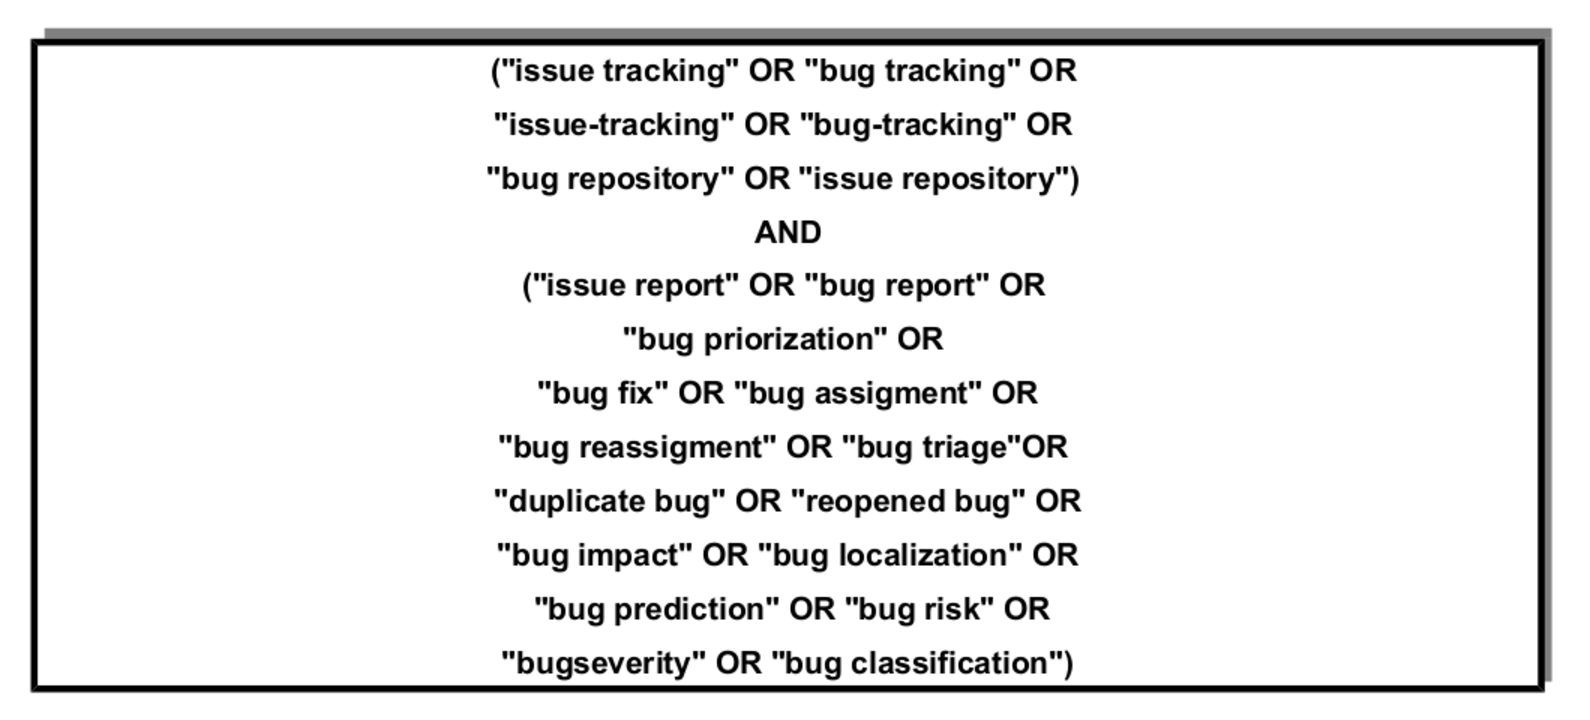
\includegraphics[width=0.8\linewidth]{./chapter-pesquisa-com-profissionais/img/setencas-grupos.pdf}
	\caption{Sentenças utilizadas para escolhas dos grupos do LinkedIn e de
		discussões no Stack Overflow}
\label{fig:setencas-grupos}
\end{figure}

\subsubsection{Estratégia de amostragem}

Apesar das Fontes de Amostragens terem sido extraídos de diferente locais, pode
ocorrer que uma sobreposição de participantes, ou seja, um mesmo participante
estar em duas ou mais fontes. Para minimizar a possibilidade da duplicação de
participação de uma mesma unidade de observação realizamos uma  desenho de
amostragem conhecido como Agrupada. Uma Amostragem agrupada pode ser aplicada
quando grupos homogêneos (clusters) compostos por unidades distintas podem ser
identificados numa população. Como consequência, devido a essa similaridade,
apenas um subconjunto desta população pode ser utilizada como amostra de forma
aleatória aleatoriamente sem perda significativa de
confiança~\cite{thompson2012sampling}. Assim, a amostragem em  agrupamentos é
comumente aplicada em pesquisas em larga escala nas quais os pesquisadores têm
restrições operacionais para recrutar e coletar
dados~\cite{roberts2004mortality}.

\subsubsection{Extração de Dados}

Para extrair os atributos necessários de cada participante desta pesquisa
utilizamos distintas. No caso da rede social Stack Overflow utilizamos uma
ferramenta da web oficial que permite compartilhar, consultar e analisar os
dados de todos os sites da rede Stack
Exchange~\footnote{\url{http://data.stackexchange.com/stackoverflow}}. A
ferramenta possibilita a utilização da linguagem SQL para acesso aos dados e
apresenta o respectivo modelo de dados para facilitar a consulta. A
Figura~\cite{fig:stack-exchange}. A ferramenta permite a extração no formato CSV
(Comma Separated Values) o qual foi inserido em um banco de dados para posterior
aplicação das regras de inclusão e exclusão.

\begin{figure}[htpb]
	\centering
	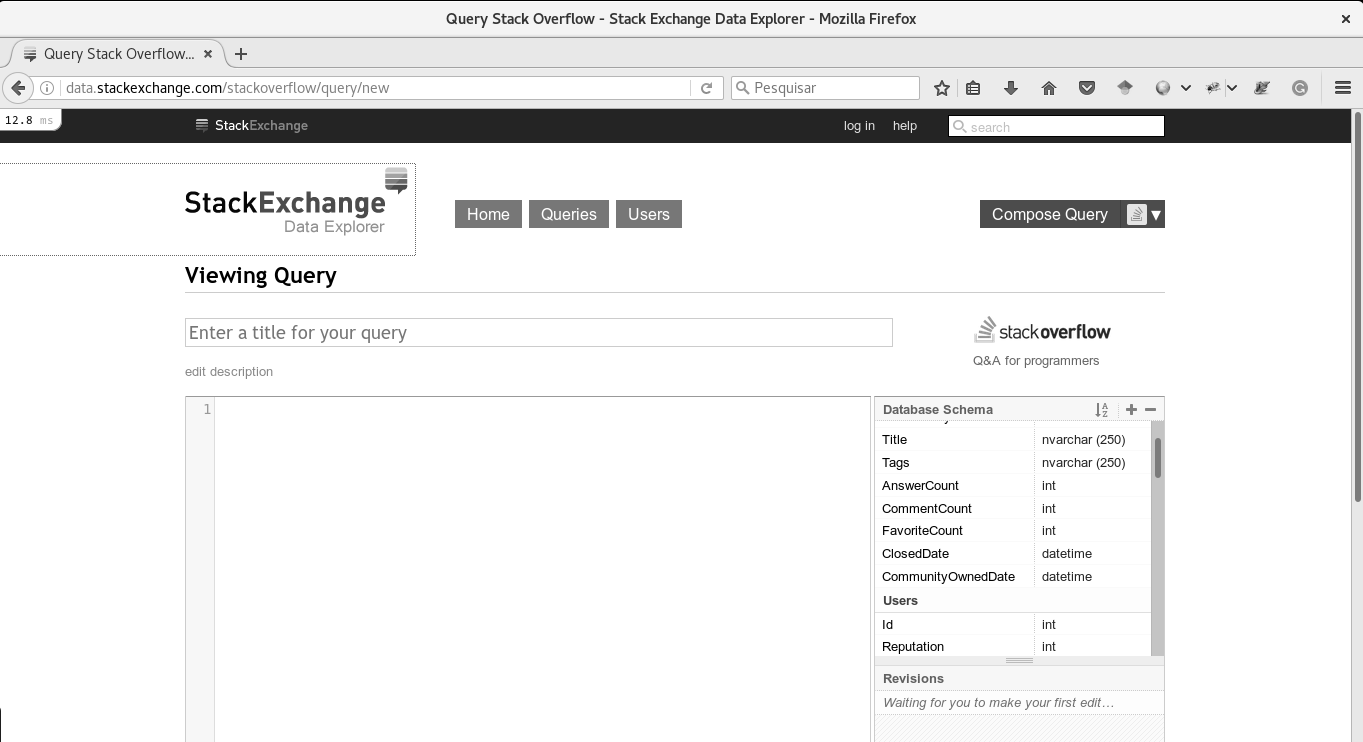
\includegraphics[width=0.8\linewidth]{./chapter-pesquisa-com-profissionais/img/stack-exchange.png}
	\caption{Ferramenta de coleta de dados da rede Stack Overflow}
\label{fig:stack-exchange}
\end{figure}

Para o projeto de código aberto desenvolvido um Web Crawler para coletar as
informações dos participantes. Um Web Crawler (rastreador web) é um programa de
computador que navega pela World Wide Web de uma forma metódica e automatizada.
A partir de uma lista de Requisições de Mudança previamente coletadas a
ferramenta coleta os dados dos participantes a partir do histórico de
modificações de determinada RM\@. A Figura~\cite{fig:historico-rm-python}
apresenta o histórico de registros de uma RM do projeto Python onde os dados dos
participantes podem ser visualizados nos quadros inseridos. A ferramenta utiliza
uma marca HTML <a> e seu valor de classe (título, ou seja, nome de membro) para
coletar os dados. De modo similar ao que foi realizados com os dados do Stack
Overflow as informações extraídas foram armazenadas em um banco de dados para
posterior aplicação de critérios de inclusão.

\begin{figure}[htpb]
	\centering
	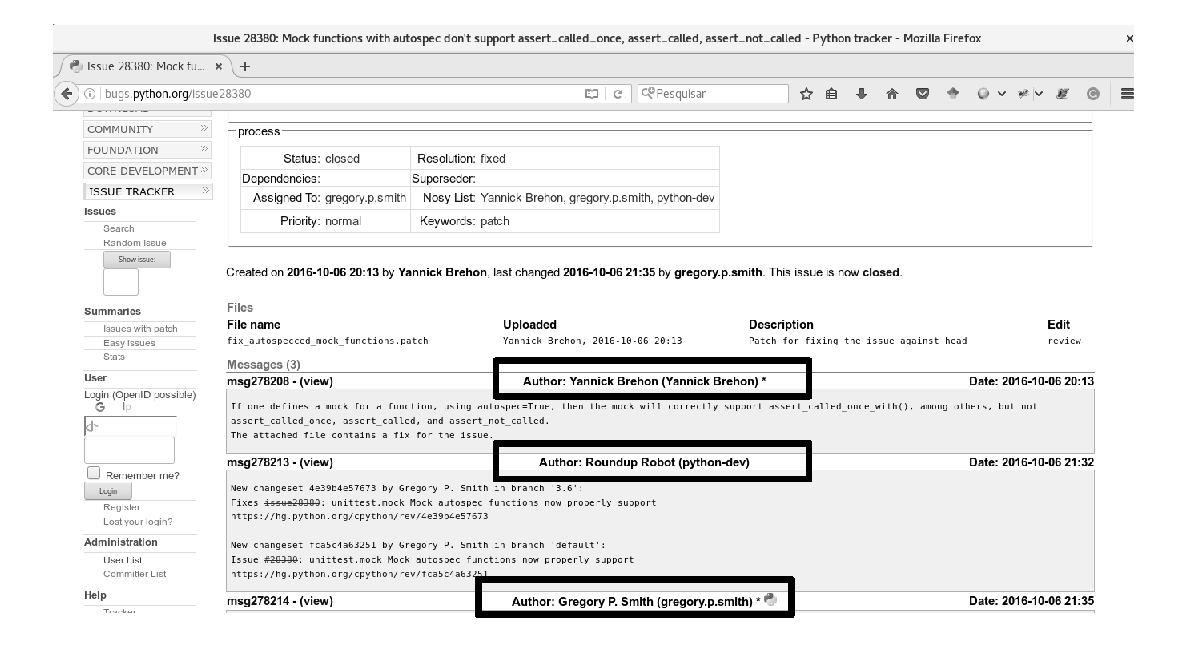
\includegraphics[width=0.8\linewidth]{./chapter-pesquisa-com-profissionais/img/historico-rm-python.pdf}
	\caption{Histórico de relatos de uma RM do projeto Python}
\label{fig:historico-rm-python}
\end{figure}

%No caso da Fonte de Amostragem do LinkedIn utilizamos a busca já existente na
%ferramenta utilizando as sentenças de busca exibidas na
%Figura~\ref{fig:setencas-grupos}. Para extrair os atributos necessários de cada
%foi utilizada uma extensão do Firefox chamada
%iMacros~\footnote{\url{http://imacros.net/}}.  Este plugin torna possível
%selecionar valores de tags HTML e salvá-los como arquivo CSV (Comma Separated
%Values). Além disso ele permite o envio de mensagem aos membros de forma
%automatizada.

%Os dados coletados nas diferentes Fontes de Amostragem foi inicialmente
%extraídos e salvos no formato CSV\@. Todavia, o arquivo CSV contém muitos dados
%indesejados e artefatos de texto que devem ser removidos. Neste caso, foi
%necessário a realização de um processo de limpeza e transformação das informação
%antes do envio propriamente dito aos participantes.

\subsubsection{Questionário}
\label{subsec:questionario}

O formulário enviado aos participantes foi estruturado em três parte, cada uma
com o objetivo de coletar um conjunto distinto de informações. Na primeira parte
estamos interessados na formação de base (background) dos profissionais. O
segundo conjunto de perguntas visa obter a percepção dos participantes sobre as
funcionalidades atualmente oferecidas pelas FGRM\@. A terceira parte é do
formulário contêm as perguntas sobre a percepção dos participantes sobre as
extensões propostas na literatura.

A fim de obtermos um formulário que conseguisse atingir os objetivos deste
estudo, realizamos um processo de avaliação em quatro etapas. O formulário
resultante de uma etapa anterior foi utilizado como entrada de uma etapa
posterior. Desta forma, utilizamos um processo iterativo para produzirmos o
formulário.
\begin{enumerate}[(i)]
	\item Avaliação por Pesquisadores: Nesta etapa o formulário inicialmente
		proposto foi enviado para dois pesquisadores experientes na área de
		manutenção de software.
	\item Avaliação por Profissionais O formulário resultante da análise
		anterior foi encaminhado a dois profissionais experientes envolvidos com
		manutenção de software.
	\item Piloto da Pesquisa O formulário obtido após a fase anterior foi
		utilizado em um piloto com
		dez profissionais envolvidos da manutenção de software de uma empresa
		pública de
		informática~-~PRODABEL\footnote{\url{{http://www.prodabel.pbh.gov.br}}}
	\item Tradução do Formulário Em cada uma das etapas de anteriores o
		formulário foi aplicado em
		português, tendo em vista que alguns profissionais envolvidos no
		processo de avaliação não
		ter fluência em língua inglesa, em especial na fase ``Piloto da
		Pesquisa'. Neste sentido, a última etapa  consistiu na tradução do
		formulário para a língua inglesa.  Esta etapa foi conduzida com  o
		suporte de um pesquisador experiente na área de Engenharia de Software.	
\end{enumerate}

\subsubsection{Envio da Mensagem}

A fim de viabilizar e mitigar os riscos operacionais do envio manual de
mensagens ao participantes foi desenvolvido um processo automatizado de envio de
mensagens ao participantes. O processo de envio seguiu uma política que consiste
em enviar uma mensagem ao participante com base em um modelo. Após um um prazo
de dois dias uma mensagem de lembrete. Foi construída uma lista para incluir os
participantes que gostariam de receber lembretes ou de participar da pesquisa de
modo a respeitar a privacidade do desenvolvedor. As mensagens foram preenchidas
(uma a uma) e enviadas através de correio eletrônico para cada um dos
participantes com base no seguinte modelo:

\fbox{\begin{minipage}{\textwidth}
Dear \{\{ nome do participante\}\}\!

I’m Vagner Clementino (\url{homepages.dcc.ufmg.br/~vagnercs}), Master Student at
Federal University of Minas Gerais, Brazil. I’m conducting a research,
supervised by Prof\. Rodolfo Resende \@-\@ \url{homepages.dcc.ufmg.br/~rodolfo}
concerned with improvements in Issue Tracking System. As part of them, we
planned and executed a survey aiming at to reach a large-scale population of
researchers/practitioners interested on to improve the features of the Issue
Tracking Systems. Based on your area of interest, we kindly invite you to take
part in the following survey:

\{\{url do formulario\}\}

You was chosen because your relevant participation/contribution in \{\{nome da
fonte de amostragem\}\}\@-\@ \{\{url da fonte de amostragem\}\}. Your opinion is
essential to strength our findings. Please, help us accordingly your
possibilities by answering this survey until \{\{data limite\}\}. As soon as we
conclude data analysis, we will share the results with all participants and the
software engineering community. If you have already fulfilled this
questionnaire, please ignore this email.

Thanks in advance,\\
Vagner Clementino\\

\end{minipage}}

\section{Resultados}
\label{sec:analise_dados}

Neste seção apresentamos os resultado obtidos da aplicação do questionário. Os
foram divididos pela questão de pesquisa ao qual visa responder. Começamos com
análise do perfil dos respondentes. Em seguida, avaliamos o nível de satisfação
que os participantes possuem com as ferramentas que eles utilizam.
Posteriormente verificamos a adoção das metodologias propostas pelos agilistas
no processo de desenvolvimento e manutenção de software. 
%Por se tratar de um estudo exploratório, no qual não foi proposta determinada
%tese a ser provada, a análise dos resultados é feita mediante o uso de gráficos
%representando a escala de Likert. Este tipo de grafo é recomendado para
%visualizar dados na escala de Likert tendo em vista que possibilita o
%entendimento da divergência entre as respostas dos
%participantes~\cite{robbins2011plotting}

\subsection{Perfil dos Participantes}
\label{sub:pesquisa_prof_perfil_dos_participantes}

Antes de apresentamos os resultado sobre as ferramentas, avaliamos o perfil dos
respondente do questionário. Como pode ser observado na
Figura~\ref{fig:grafico_melhorias_fgrm_funcao_particantes} a função mais
frequente é a de desenvolvedor. Todavia grande parte dos respondentes estão
diretamente vinculado ao desenvolvimento e manutenção de software, tanto que
mais de 80\% é formado por desenvolvedores, engenheiros de software, gerentes e
arquitetos. 

\begin{figure}[htpb]
	\centering
	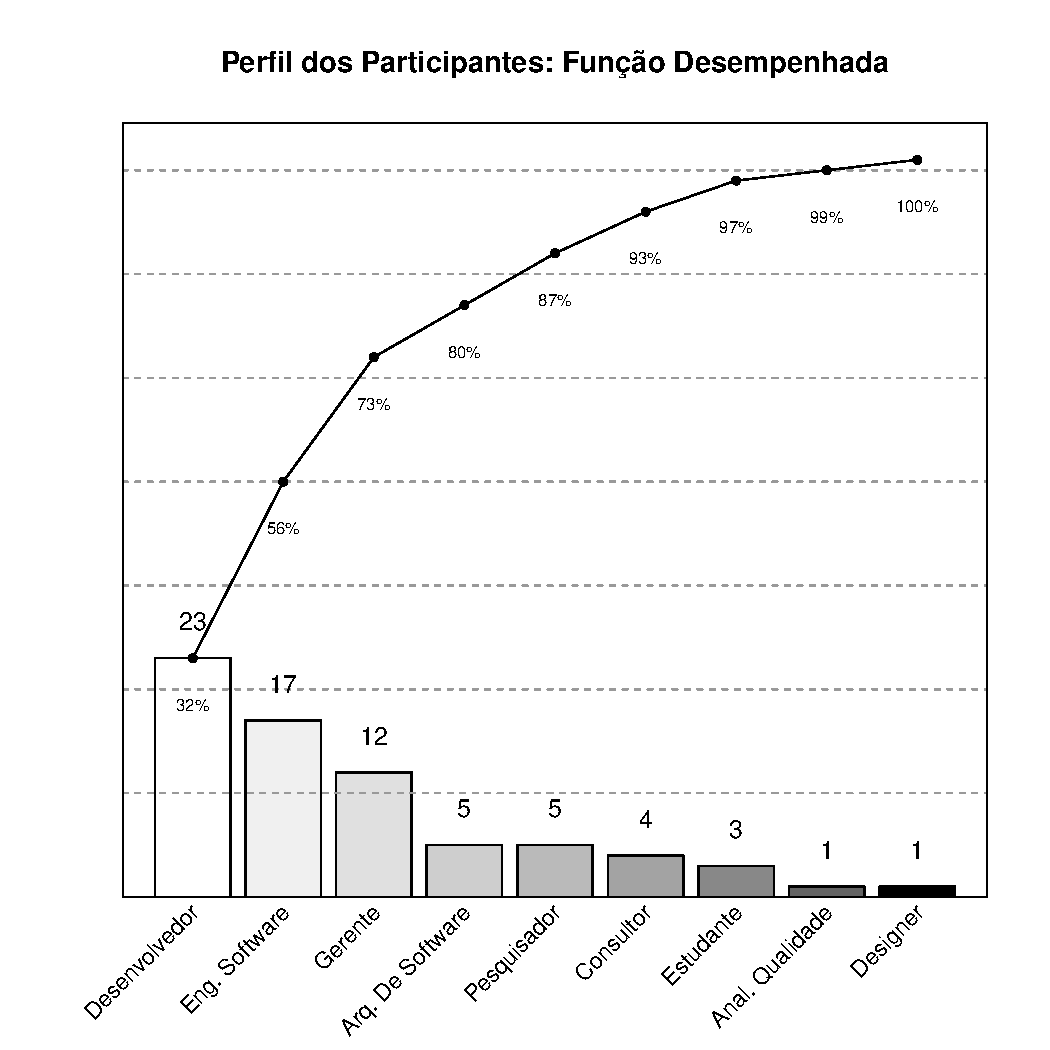
\includegraphics[width=0.8\linewidth]{./chapter-pesquisa-com-profissionais/img/grafico_melhoria_fgrm_funcao_participantes.pdf}
	\caption{Função dos Participantes}
\label{fig:grafico_melhorias_fgrm_funcao_particantes}
\end{figure}

A distribuição geográfica dos participantes pode ser visualizada na
Figura~\ref{fig:grafico_melhorias_fgrm_localizacao_geografica}. Há uma
proeminência de pessoas da Ásia e Europa e posteriormente das Américas. Esta
distribuição pode minimizar possíveis enviesamentos que por ventura algum nicho
geográfico possa apresentar. Todavia, não está no escopo deste estudo discutir
as diferenças que a localização do participante influencia aos resultados. 

\begin{figure}[htpb]
	\centering
	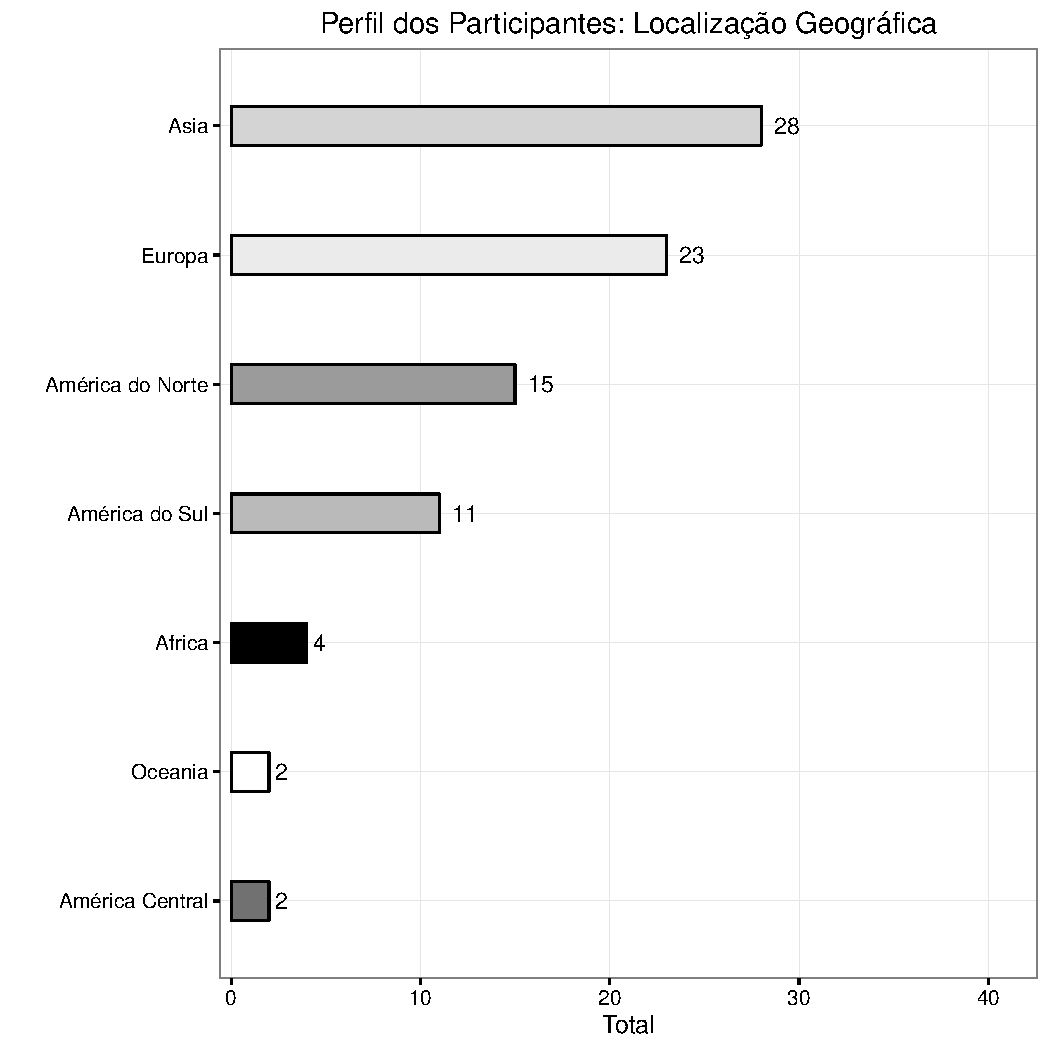
\includegraphics[width=0.8\linewidth]{./chapter-pesquisa-com-profissionais/img/grafico_melhorias_fgrm_localizacao_geografica.pdf}
	\caption{Localização Geográfica dos Participantes}
\label{fig:grafico_melhorias_fgrm_localizacao_geografica}
\end{figure}

Os respondentes trabalham em sua maioria em empresas privadas de software.
Existem também aqueles que participam de projetos de código aberto. A
distribuição do local do participante pode ser vista na
Figura~\cite{fig:grafico_melhorias_fgrm_local_trabalho}. É importante considerar
que grande parte dos respondentes pertencem à empresas privadas, onde os
processos e ferramentas não podem ser modificados pelo desenvolvedor. Esta
característica dos participantes pode afetar os resultados, especialmente quando
	avaliarmos o nível de satisfação com as FGRM's. 

\begin{figure}[htpb]
	\centering
	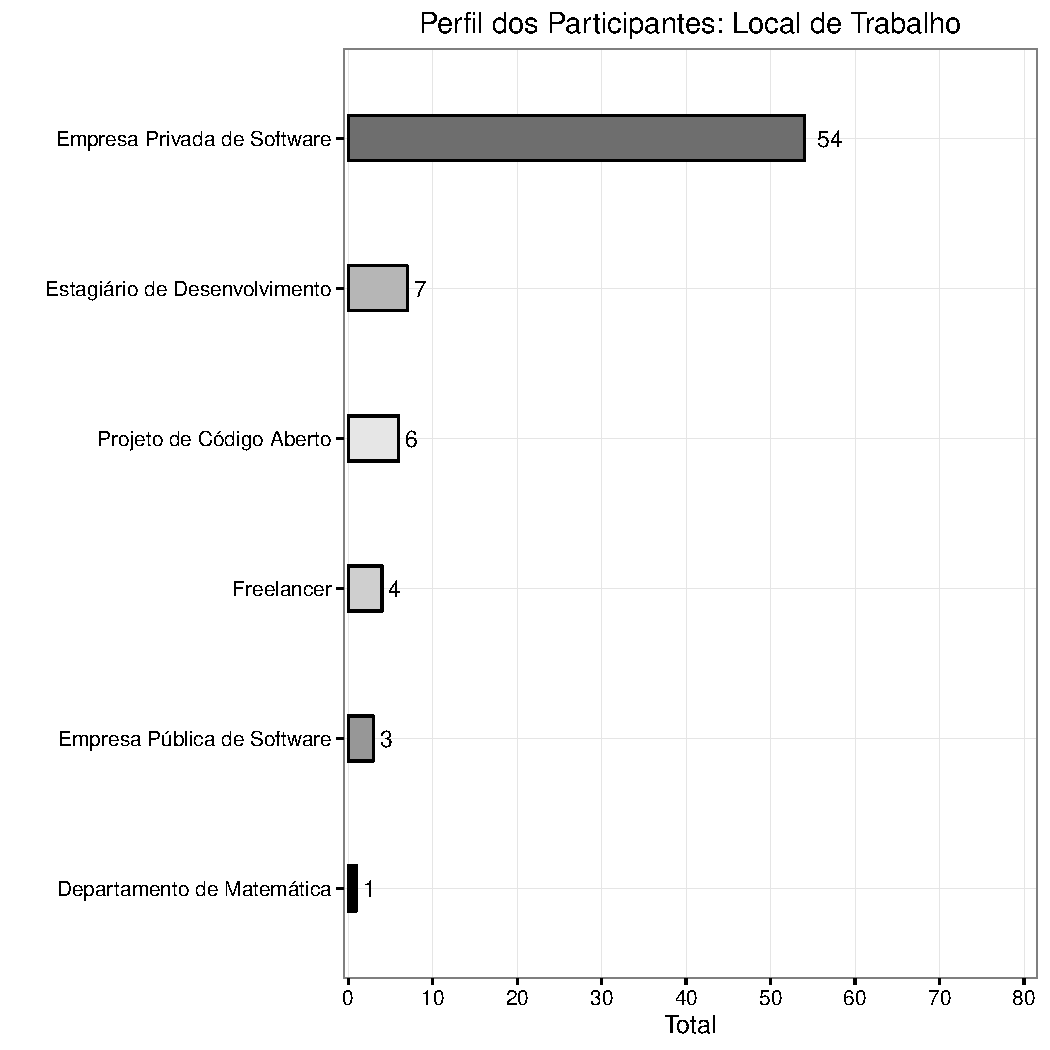
\includegraphics[width=0.8\linewidth]{./chapter-pesquisa-com-profissionais/img/grafico_melhorias_fgrm_local_trabalho.pdf}
	\caption{Local de Trabalho}
\label{fig:grafico_melhorias_fgrm_local_trabalho}
\end{figure}

No tocante ao tamanho da equipe ao qual o participante faz parte verificamos a
predominância de um número com mais de seis membros, conforme pode ser observado
na Figura~\ref{fig:grafico_melhorias_fgrm_tamanho_equipe}. Apesar da maior
frequência de respostas é para equipes de tamanho maior do que dez membros,
acreditamos que o número de membros não seja muito maior do que isso.

\begin{figure}[htpb]
	\centering
	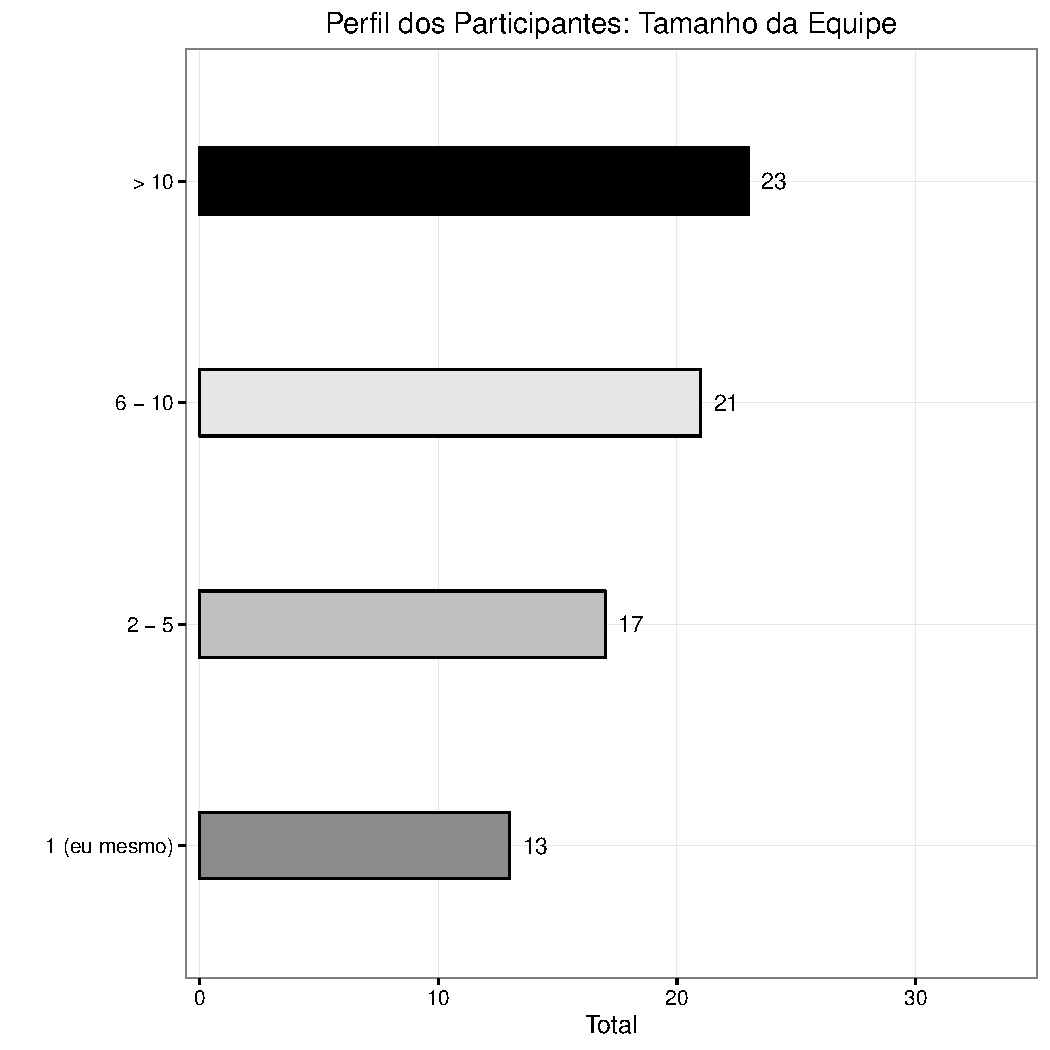
\includegraphics[width=0.8\linewidth]{./chapter-pesquisa-com-profissionais/img/grafico_melhorias_fgrm_tamanho_equipe.pdf}
	\caption{Tamanho da Equipe}
\label{fig:grafico_melhorias_fgrm_tamanho_equipe}
\end{figure}

Os participantes possuem com maior frequência entre três e dez anos. Existem
ainda um grupo significativo (09 participantes) que possuem mais de dez anos de
experiência. Em síntese, temos um grupo com significativa experiência o que pode
agregar valor aos resultados finais. A distribuição do tempo de experiência pode
ser visualizado na Figura~\ref{fig:grafico_melhorias_fgrm_tempo_experiencia}.

\begin{figure}[htpb]
	\centering
	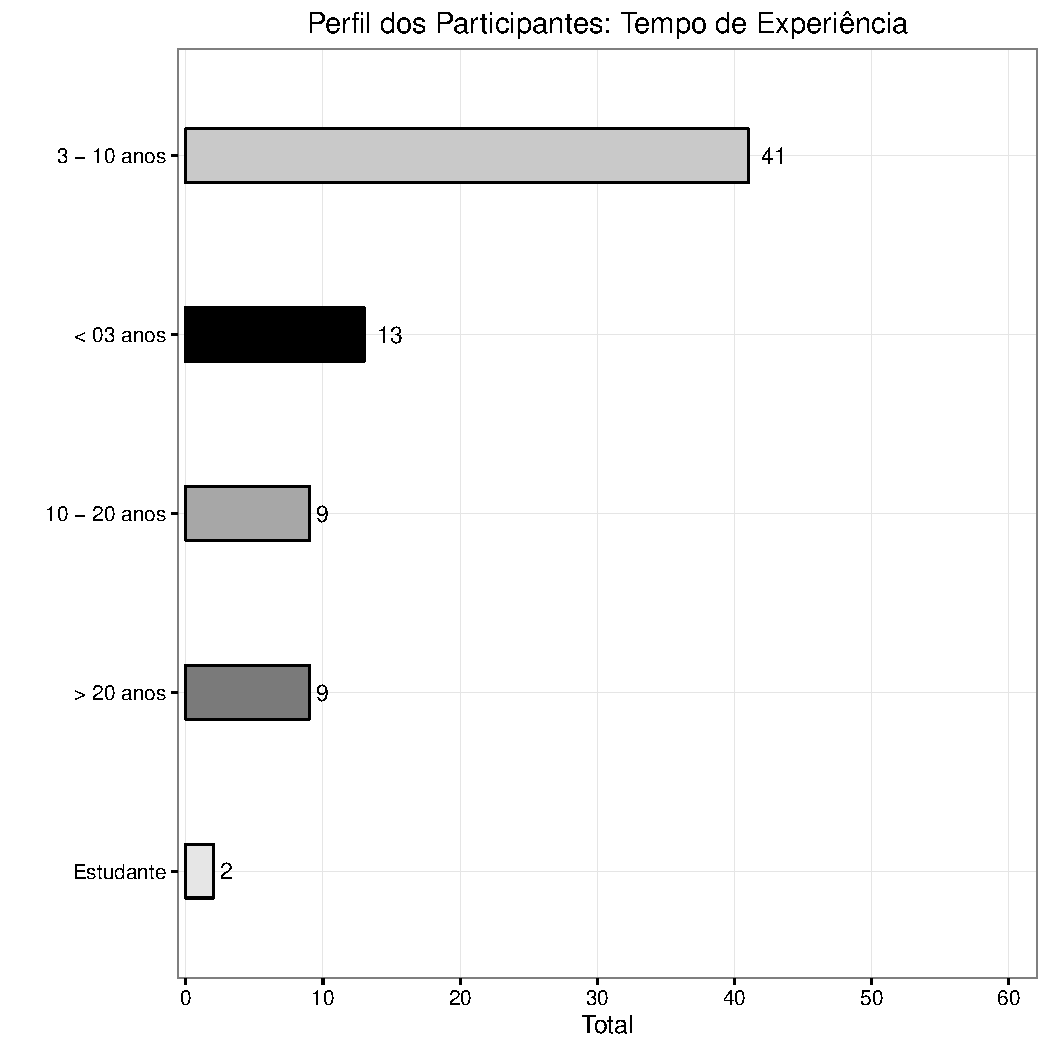
\includegraphics[width=0.8\linewidth]{./chapter-pesquisa-com-profissionais/img/grafico_melhorias_fgrm_tempo_experiencia.pdf}
	\caption{Tempo de Experiência}
\label{fig:grafico_melhorias_fgrm_tempo_experiencia}
\end{figure}

Em resumo as respostas vieram de desenvolvedores, localizados na Ásia e Europa,
com um tempo de experiência entre três e dez anos, trabalhando em uma equipe com
aproximadamente dez membros. A partir deste perfil entendemos que conseguimos
alcançar uma amostra com um perfil suficiente para responder as questões
propostas.

\subsection{Nível de Satisfação com as FGRM}
\label{sub:nivel_de_satisfação_com_as_fgrm}

Para respondermos a Questão de Pesquisa é importante analisarmos as ferramentas
utilizadas pelos profissional que respondeu a pesquisa. Esta informação é
importante tendo que vista que as opiniões dadas pelos participantes estão
diretamente relacionada com a versão utilizada, podendo os resultados se
mostrarem diferentes se a pesquisa fosse realizada com outra versão dos sistema.
A Figura~\ref{fig:grafico_melhorias_fgrm_ferramentas_utilizadas} exibe as
ferramentas utilizadas pelos profissionais que responderam ao questionário. A
maior frequência na ferramenta \textit{Jira} que é uma FGRM que integra em seu
processo de gestão das RM's métodos propostos pelos agilistas. Na segunda
posição visualizamos o Github que é um serviço de web para armazenamento para
projetos que usam o controle de versionamento \textit{Git} e possui uma FGRM
integrada.

\begin{figure}[htpb]
	\centering
	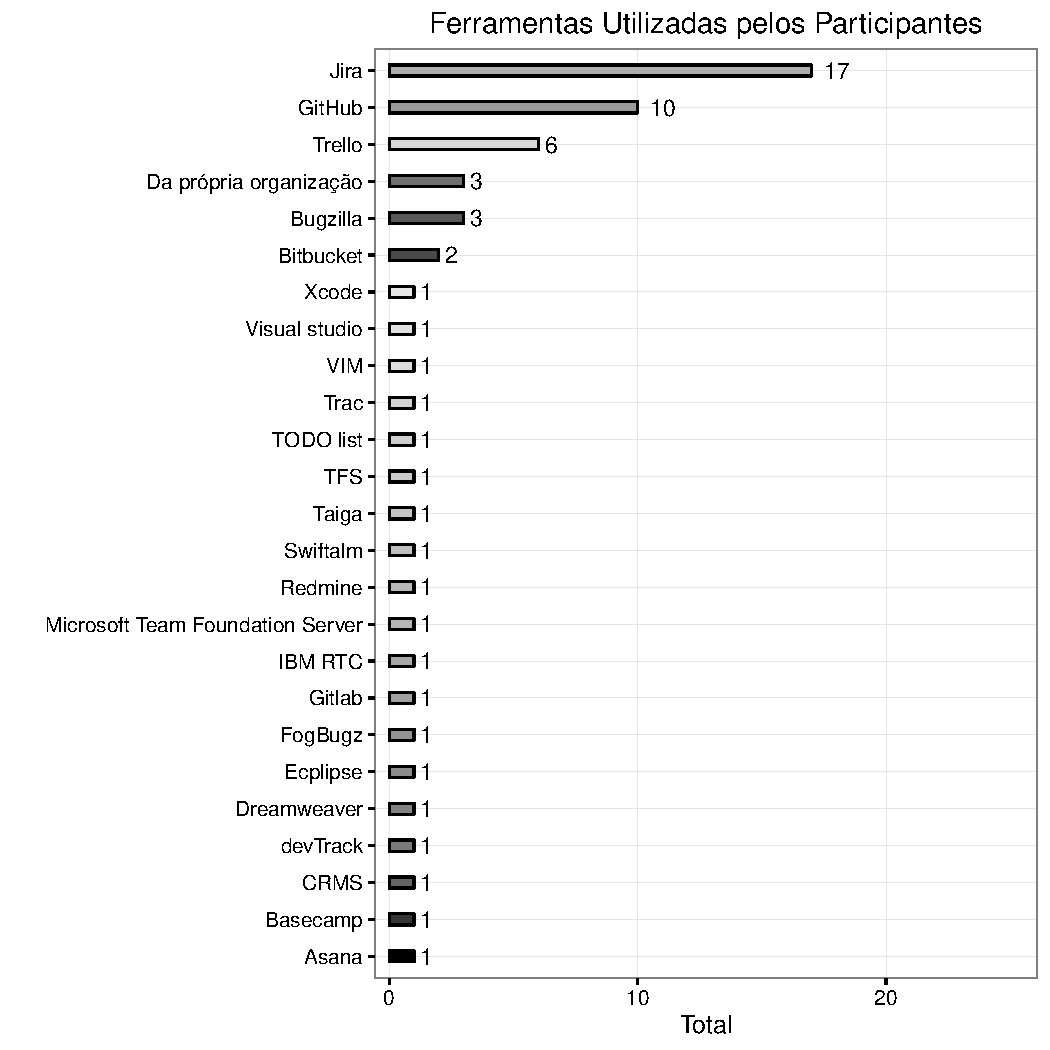
\includegraphics[width=0.8\linewidth]{./chapter-pesquisa-com-profissionais/img/grafico_melhorias_fgrm_ferramentas_utilizadas.pdf}
	\caption{Ferramentas utilizadas pelos participantes}
\label{fig:grafico_melhorias_fgrm_ferramentas_utilizadas}
\end{figure}

Inicialmente gostaríamos de saber qual o nível de satisfação com os participantes
com as funcionalidades pelas FGRM que ele utiliza atualmente. Esta medida pode
ser visualizada na Figura~\ref{grafico_melhorias_fgrm_nivel_satisfacao}. Em
grande parte os respondentes estão satisfeitos com as funcionalidades. A
resposta com maior frequência foi \textit{OK}, o que pode ser visto que este
tipo de software está atualmente atendendo as expectativas de seus usuários.
Este resultado não segue o que literatura da área discute, onde este tipo de
ferramenta é vista com necessidade de melhora, tomando com base a visão dos
profissionais. Esta aparente dicotomia pode ser justificada, possivelmente, pelo
desconhecimento dos profissionais de funcionalidades que estão sendo propostas
na literatura que podem melhorar as suas atividades diárias.
\begin{figure}[htpb]
	\centering
	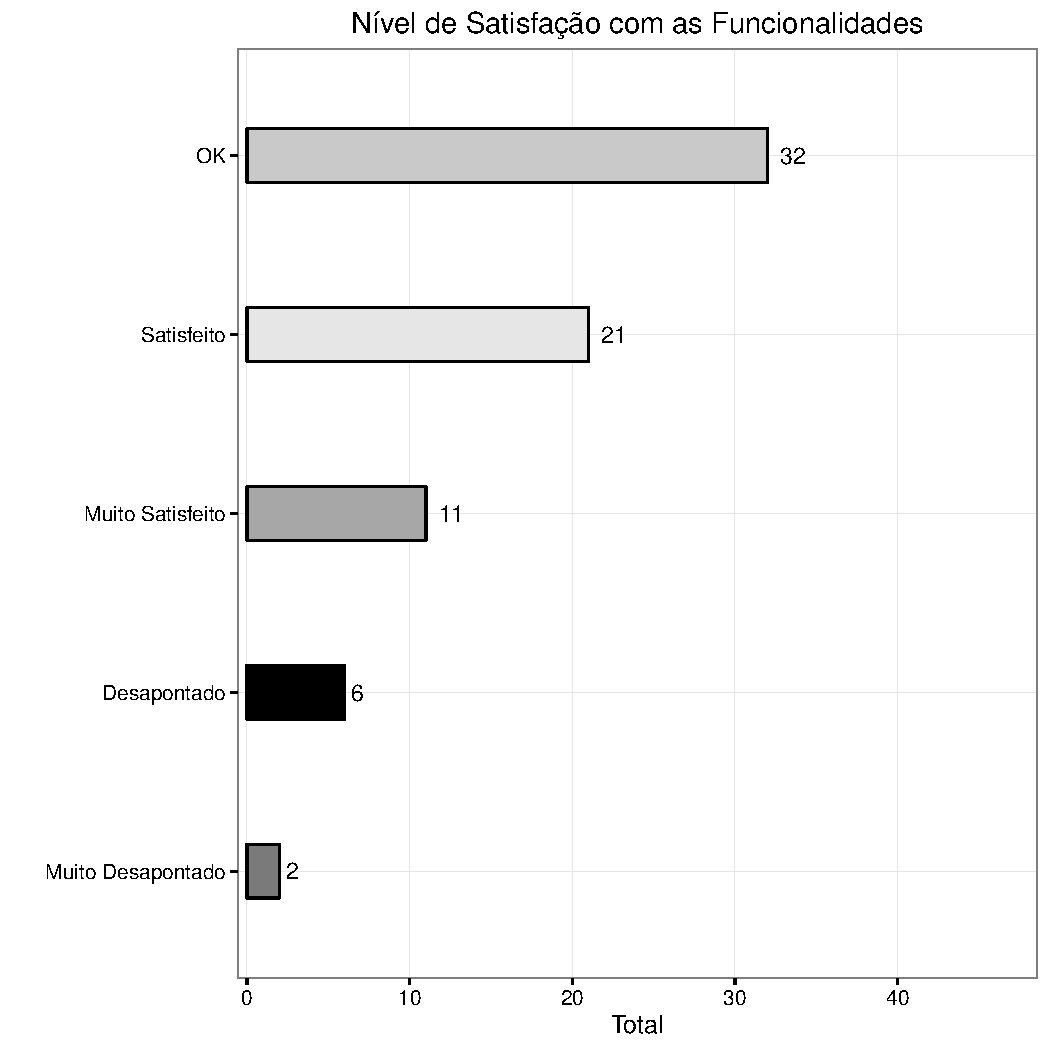
\includegraphics[width=0.8\linewidth]{./chapter-pesquisa-com-profissionais/img/grafico_melhorias_fgrm_nivel_satisfacao.pdf}
	\caption{Nível de satisfação com as Ferramentas}
\label{fig:grafico_melhorias_fgrm_nivel_satisfacao}
\end{figure}

No mesmo questionário verificamos junto aos profissionais se eles recomendariam
a ferramenta que utiliza atualmente para um outro projeto. A probabilidade de
recomendação é exibida na
Figura~\ref{fig:grafico_melhorias_fgrm_probabilidade_recomentacao}. De maneira
similar ao nível de satisfação grande parte dos participantes tendem a
recomendar a FGRM que utiliza para um novo projeto. Com base neste resultado
podemos deduzir que os profissionais estão realmente satisfeitos comas
funcionalidades da ferramenta que utiliza ao ponto de recomendá-la.

\begin{figure}[htpb]
	\centering
	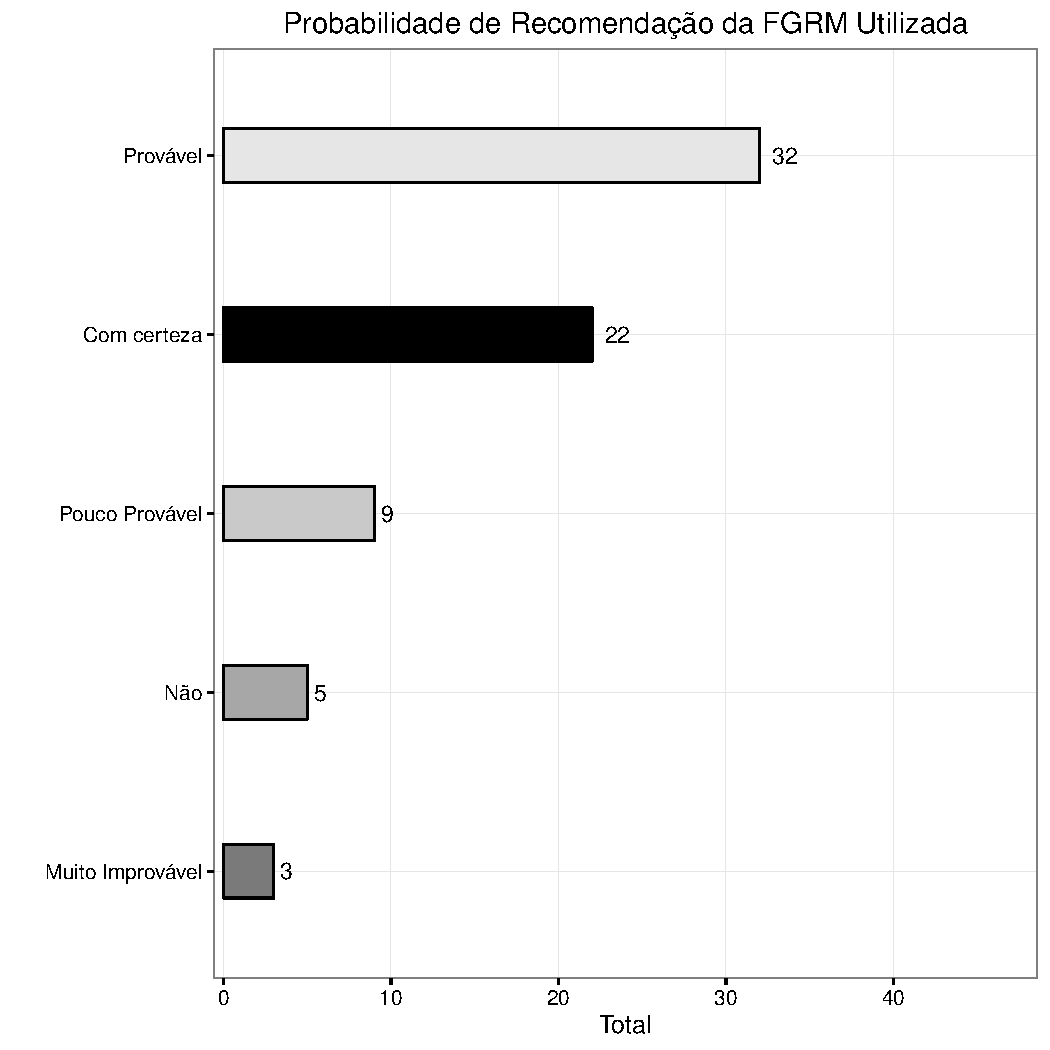
\includegraphics[width=0.8\linewidth]{./chapter-pesquisa-com-profissionais/img/grafico_melhorias_fgrm_probabilidade_recomentacao.pdf}
	\caption{Probabilidade de Recomendação da Ferramenta Utilizada}
\label{fig:grafico_melhorias_fgrm_probabilidade_recomentacao}
\end{figure}

\subsection{Avaliação das Funcionalidades Existentes}
\label{sub:avaliação_das_funcionalidades_existentes}

Nesta seção apresentamos a opinião dos profissionais envolvidos em Manutenção de Software com relação as
funcionalidades oferecidas atualmente pelas FGRM\@. Este ponto de vista pode ser
visualizado na Tabela~\ref{tab:avaliacao_funcionalidades}. É possível verificar
que os profissionais avaliaram como importantes funções como \textit{Suporte ao
Unicode, Múltiplos Projetos, Integração com Sistemas de Controle de Versão (VCS
Integration)} como  funções importantes em sua atividades diárias. 

\begin{table}[htpb]
\centering
\resizebox{\textwidth}{!}{%
\begin{tabular}{|l|c|c|c|c|c|}
\hline
\multicolumn{1}{|c|}{\multirow{2}{*}{\textbf{Funcionalidade}}} & \multicolumn{5}{c|}{\textbf{Classificação}} \\ \cline{2-6} 
\multicolumn{1}{|c|}{} & \textbf{Not at all important} & \textbf{Slightly Important} & \textbf{Important} & \textbf{Fairly Important} & \textbf{Very Important} \\ \hline
Documentation integration/generation, business reporting & 11 & 12 & 15 & 12 & 14 \\ \hline
Test planning integration & 11 & 13 & 13 & 13 & 9 \\ \hline
Customizable workflow & 9 & 14 & 21 & 14 & 15 \\ \hline
Unicode support & 9 & 9 & 21 & 16 & 24 \\ \hline
Custom fields & 5 & 17 & 25 & 22 & 8 \\ \hline
Support to Service Level Agreement & 14 & 22 & 15 & 13 & 10 \\ \hline
Plugin API to integration with other products & 8 & 14 & 21 & 19 & 16 \\ \hline
Multiple projects & 3 & 8 & 17 & 21 & 28 \\ \hline
Full-text search & 1 & 5 & 17 & 15 & 40 \\ \hline
File search & 4 & 15 & 18 & 17 & 24 \\ \hline
VCS integration & 7 & 16 & 16 & 13 & 21 \\ \hline
Multiples interfaces of notifications (E-mail, RSS, XMPP, etc) & 7 & 11 & 23 & 16 & 19 \\ \hline
Code Review Support & 2 & 2 & 0 & 0 & 5 \\ \hline
Ease of use & 0 & 2 & 2 & 0 & 1 \\ \hline
Integration with database \& app & 4 & 6 & 4 & 1 & 2 \\ \hline
Reviewing & 0 & 4 & 10 & 6 & 1 \\ \hline
User Experience and Ease of Use & 2 & 4 & 0 & 6 & 3 \\ \hline
Git branch style & 10 & 2 & 2 & 3 & 2 \\ \hline
\end{tabular}%
}
\caption{Avaliação das funcionalidades das FGRM's do ponto de vista dos
	profissionais.}
\label{tab:avaliacao_funcionalidades}
\end{table}

Por outro apresentamos aos profissionais funcionalidades que poderiam ser
integradas à FGRM que ele utiliza. A opinião dos participantes pode ser
visualizada na Figura~\ref{fig:ggrafico_melhorias_fgrm_melhorias}. Conforme pode
ser observado que melhorias na busca de busca de RM's, coleta de informações
para solucionar na resolução da RM e dar suporte ao registro de RM's como
funcionalidades que podem melhorar as atividades do desenvolvedor.

\begin{figure}[htpb]
	\centering
	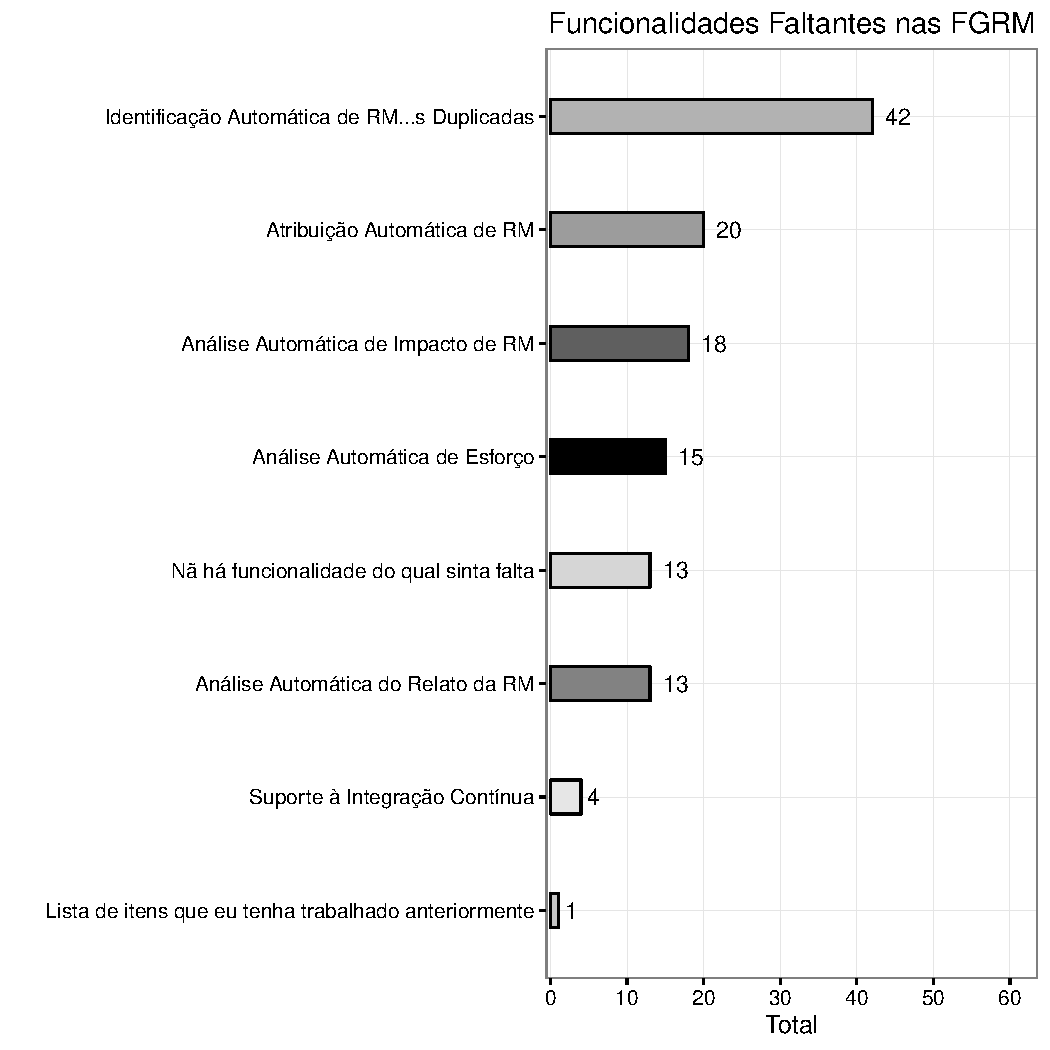
\includegraphics[width=0.8\linewidth]{./chapter-pesquisa-com-profissionais/img/grafico_melhorias_fgrm_funcionalidades_faltantes.pdf}
	\caption{Funcionalidades que o participantes sentem falta.}
	\label{fig:grafico_melhorias_fgrm_funcionalidades_falantes}
\end{figure}

Por outro lado algumas das melhorias propostas na literatura se mostram de
interesse pelos profissionais. A
Figura~\ref{fig:grafico_melhorias_fgrm_funcionalidades_falantes} apresenta as
funcionalidades que os participantes sentem falta. Funções tais como
identificação automática de RM's duplicadas, atribuição automática de RM e
Análise de Impacto foram as mais frequentes. 

\begin{figure}[htpb]
	\centering
	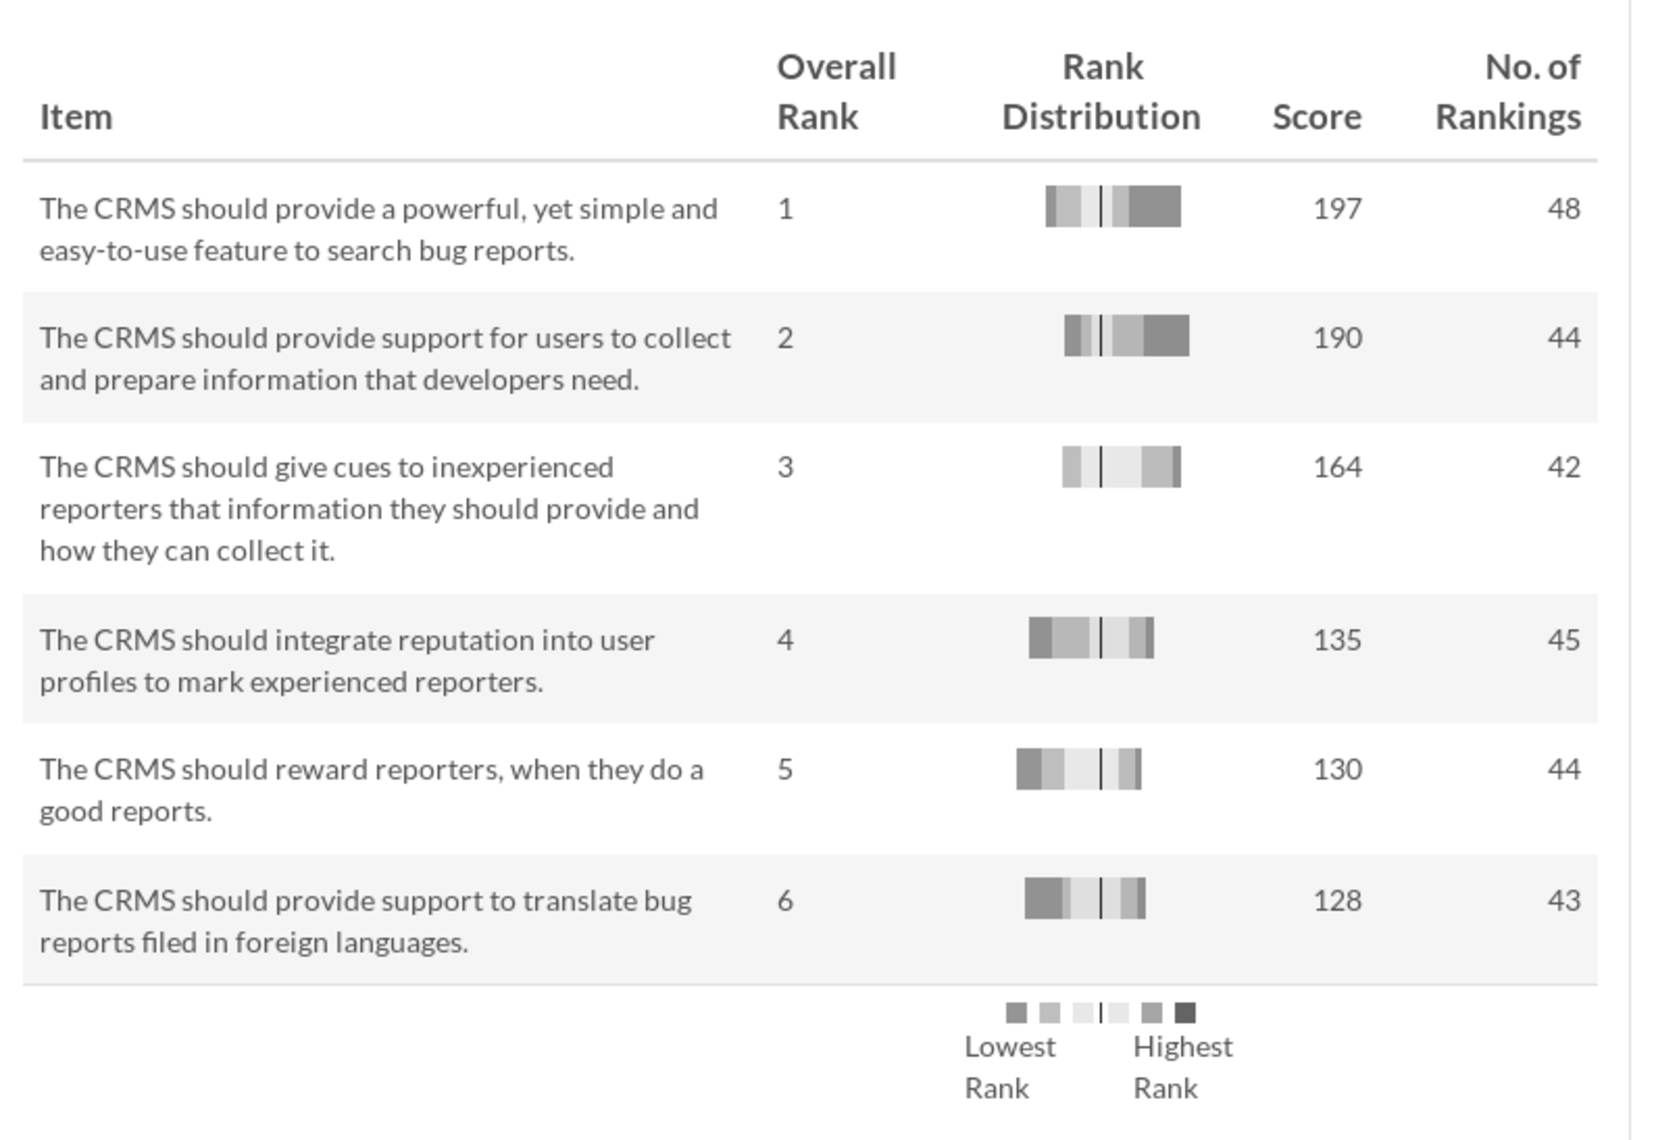
\includegraphics[width=0.8\linewidth]{./chapter-pesquisa-com-profissionais/img/grafico_melhorias_fgrm_melhorias.pdf}
	\caption{Novas funcionalidades para as FGRM's.}
	\label{fig:ggrafico_melhorias_fgrm_melhorias}
\end{figure}


\subsection{Práticas Ágeis na Manutenção de Software}
\label{sub:práticas_ágeis_na_manutenção_de_software}

Nesta etapa deste estudos estamos interessados como as práticas propostas pelos
agilistas estão sendo utilizadas especialmente no processo de manutenção de
software. A Figura~\ref{fig:grafico_melhorias_fgrm_praticas_ageis_adotadas}
exibe as metodologias ágeis que estão sendo utilizadas durante o processo de
manutenção de software. As práticas mais adotadas são Integração Contínua,
Padrões de Programação e Refatoração são práticas adotadas quando da realização
desta pesquisa. 

\begin{figure}[htpb]
	\centering
	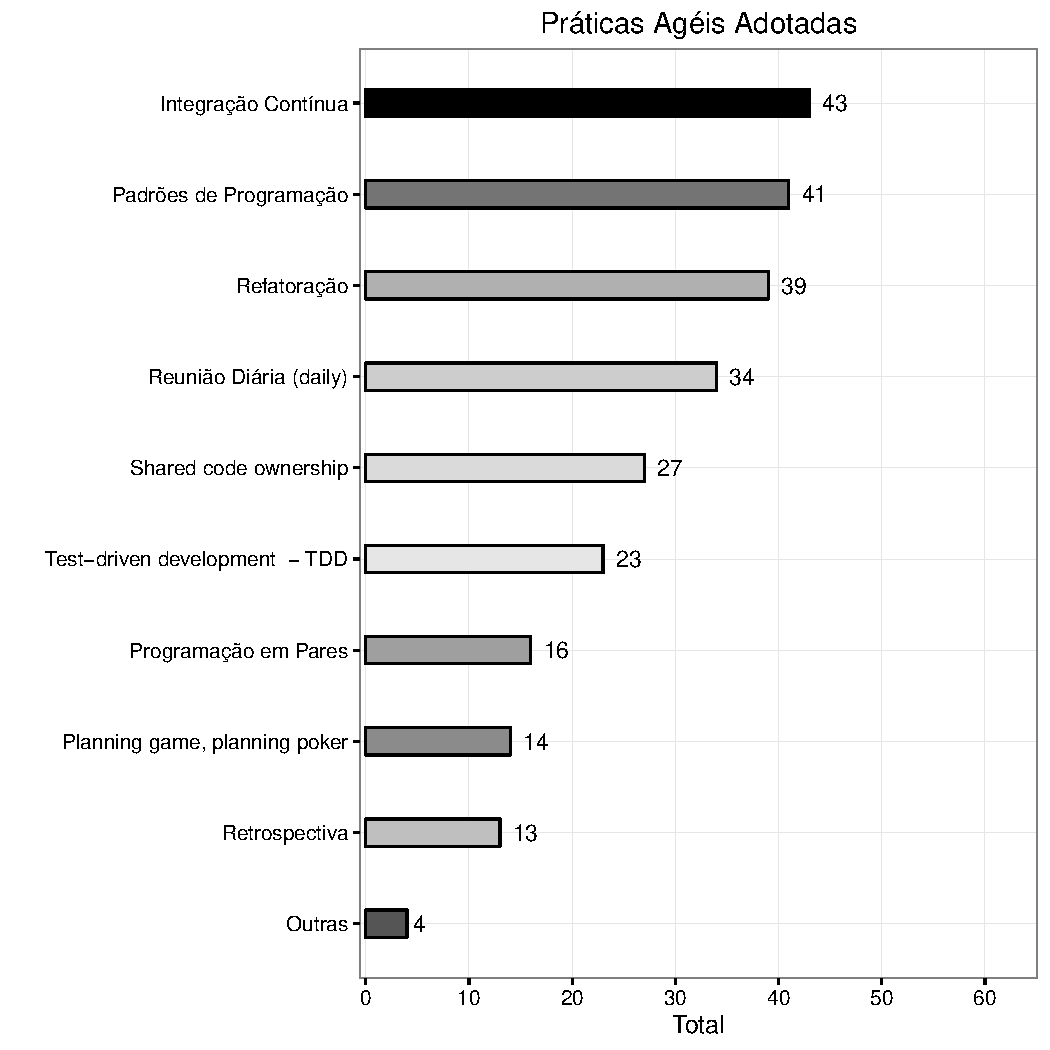
\includegraphics[width=0.8\linewidth]{./chapter-pesquisa-com-profissionais/img/grafico_melhorias_fgrm_praticas_ageis_adotadas.pdf}
	\caption{Metodologias propostas pelos agilistas que são adotadas pelos
		participantes.}
	\label{fig:grafico_melhorias_fgrm_praticas_ageis_adotadas}
\end{figure}

A fim de avaliar como as FGRM's podem ajudar aos times devotados à manutenção de
software na prática adotada pelos agilistas apresentamos uma lista de possíveis
funcionalidades que este tipo de ferramenta poderia fornecer. A
Figura~\ref{fig:grafico_melhorias_fgrm_suporte_particas_ageis} apresenta a
opinião dos profissionais quais as funcionalidades seriam mais relevantes.
Segundo a opinião dos participantes a priorização automática de RM's urgente e
não esperadas, ajuda do desenvolvedor em sua reunião diária (daily) e o suporte
a tarefas compartilhadas foram as mais frequentes. 

\begin{figure}[htpb]
	\centering
	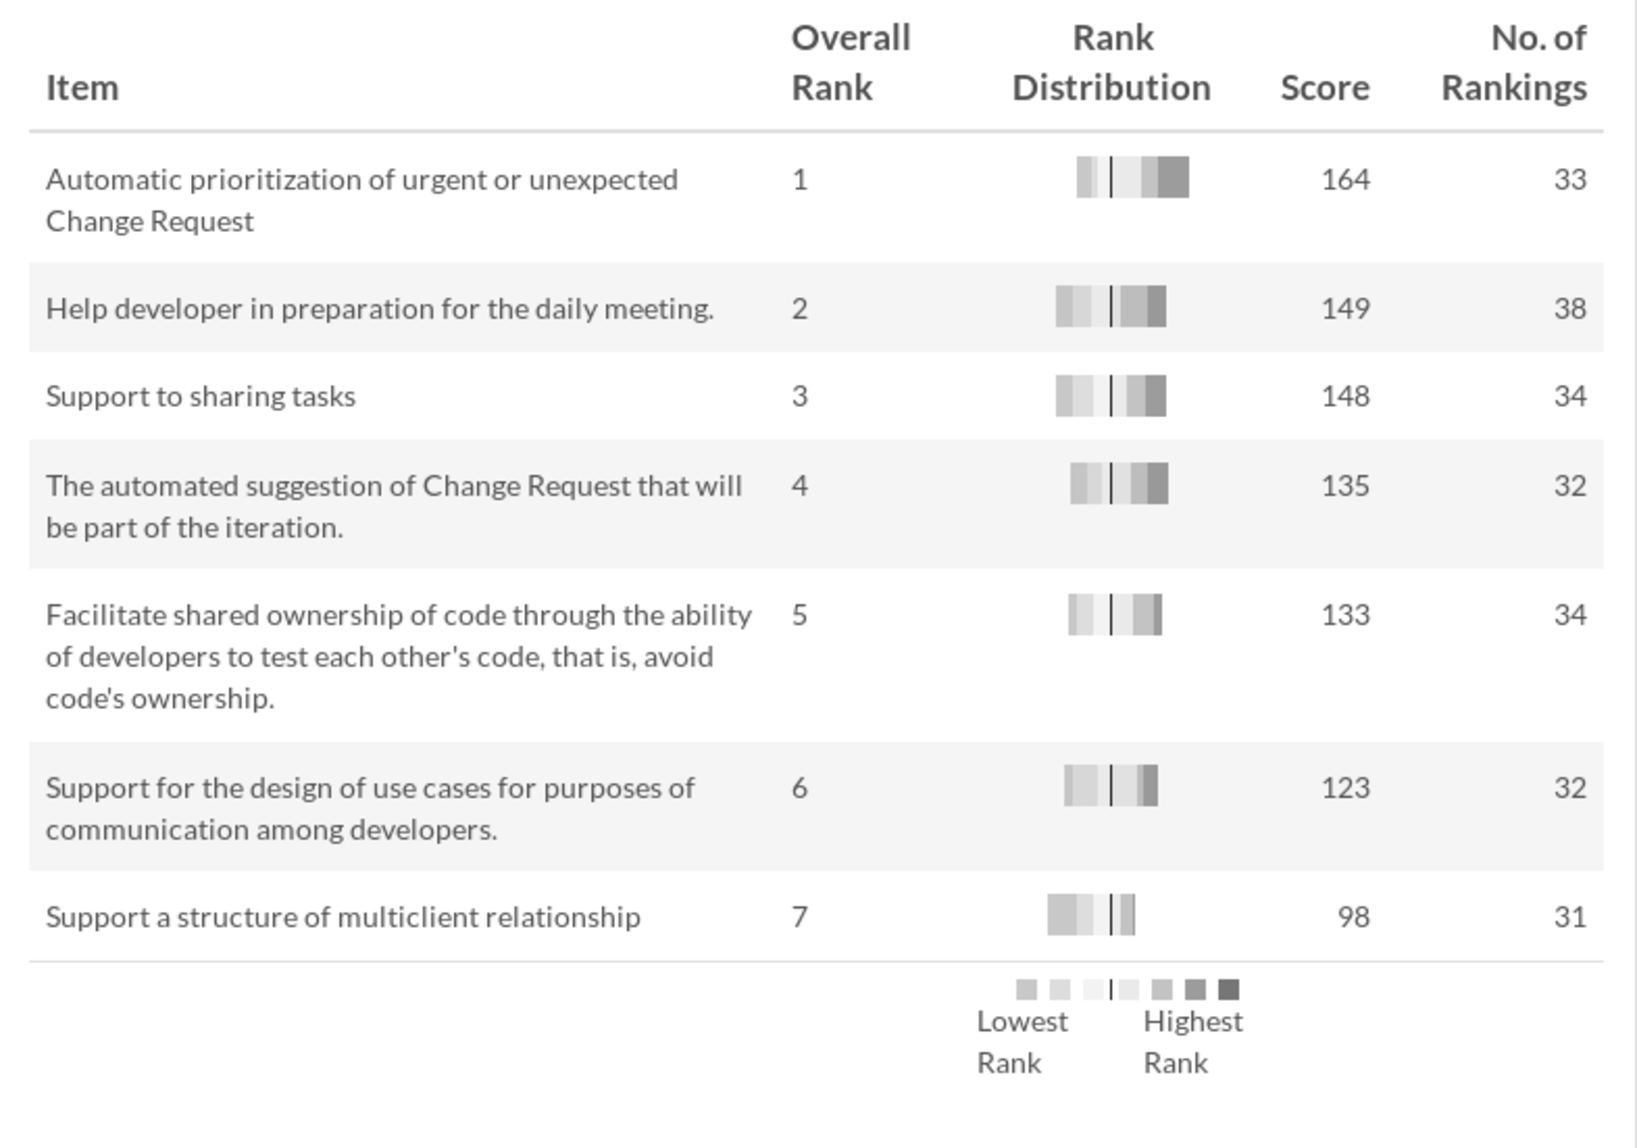
\includegraphics[width=0.8\linewidth]{./chapter-pesquisa-com-profissionais/img/grafico_melhorias_fgrm_suporte_particas_ageis.pdf}
	\caption{Classificação das funcionalidades que possam dar suporte ao uso das
	metodologias dos agilistas.}
	\label{fig:grafico_melhorias_fgrm_suporte_particas_ageis}
\end{figure}

\section{Discussão}

\paragraph{Nível de Satisfação com a Ferramenta Utilizada.}
\label{par:pesq_profissionais_nivel_de_satisfação}

Em geral, o nível de satisfação com as funcionalidades oferecidas pelas FGRM's é
alto. Esta medida foi observada no
Figura~\ref{fig:grafico_melhorias_fgrm_nivel_satisfacao} no qual verificamos que
cerca de 90\% dos participantes estão de alguma forma satisfeito com a
ferramenta utilizada diariamente. Este mesmo sentimento pode ser observado pela
probabilidade de recomendação do sistema que utilizada para um novo projeto.
Naquela medida verificamos que o mesmo percentual de participantes pretendem
recomendar o software que utiliza.

\paragraph{Funcionalidades Faltantes.}
\label{par:pesq_profissionais_funcionalidades_faltantes}




\section{Ameças à Validade}
As ameaças à validade deste trabalho está principalmente no numero de
respondentes da pesquisa. Apesar de ter sido realizada uma seleção metodológica
de uma amostra representativa da população o número de participantes limita a
extrapolação do resultados obtidos. Da mesma forma, todas as opiniões coletadas
devem sempre levar em conta a ferramenta que o profissional utilize quando da
aplicação do questionário. Caso este mesmo estudo fosse realizado com outras
versões do mesmos sistemas os resultados poderiam ser diferentes. Neste sentido,
a generalização dos resultados também passa por esta característica do estudo.


%\section{Resumo do Capítulo}
\label{sec:resumo_do_capitulo}
